\documentclass{beamer}
\usetheme{metropolis} 
\usecolortheme{rose}

\usepackage{xcolor}
\usepackage[utf8]{inputenc}
\usepackage{hyphenat}
\usepackage[russian,english]{babel}          % Use metropolis theme
\usepackage{wrapfig}

\setbeamertemplate{footline}[frame number] % указывает на каждой странице общее количество страниц

% Указывайте все новые термины в \termdef команде. А уже известные ранее или из других курсов в \term
\newcommand{\termdef}[1]{\textbf{\textit{#1}}}
\newcommand{\term}{\textit}
% Диалог с аудиторией.
\newcommand{\auditorium}[1]{\color{red}{\textbf{#1}}}
% \setbeamercolor{auditorium}{fg=red}

\title{Лекция 3. Дерево решений. Лес. Случайный лес}
% \date{\today}
\date{1 октября 2019}
\author{Павел Владимирович Слипенчук}
\institute{Москва, МГТУ им.Бауманка,\\ каф.ИУ-8, КИБ}
% \titlegraphic{\includegraphics[width=2cm]{logo_ur.jpg}}
\titlegraphic{\small \href{https://github.com/kib-courses/dsis}{Data Science для решения задач информационной безопасности}}

\begin{document}
  \maketitle
    
  \begin{frame}{План лекции}
    \begin{enumerate}
	 \item \nameref{section:tree_forest}
	 \item \nameref{section:random_tree_building}
	% \item \nameref{section:precision_recall_defs}
	% \item \nameref{section:all_of_them}
	\end{enumerate}
 \end{frame}
    
  \begin{frame}
  \begin{block}{Замечание}
  	Алгоритмов машинного обучения очень много. 
  	Хороший Data Scientist должен взять себе в привычку
  	время от времени изучать те или иные алгоритмы.
  	
  	Цель курса -- прикладная. Научить решать ИБ задачи с помощью
  	Data Science методов.
  	
  	Тем не менее хотя бы один алгоритм должен быть изучен.
  \end{block}
 \end{frame}
  \begin{frame}
  \termdef{Случайный лес}(Random Forest, RF) -- это легко объясняемый, 
  понятный, 
  устойчивый к переобучению (overfitting)
  алгоритм ML.
  
  RF является мощным средством против <<активного противника>>\footnote{
  в задачах с обратной связью изучаемого субъекта (хакера, мошенника)
  }. 

  Вопреки высасаным из пальца примерам, на реальныхъ данных
  RF всегда работает, если признаки информативны и "неразряжены".
  \end{frame}

   \section{Дерево решений. Лес решений}\label{section:tree_forest}
	

  \begin{frame}{Дерево решений}
  
  Отрывок из <<Choosing the right estimator>>:\footnote{\tiny \url{https://scikit-learn.org/stable/tutorial/machine_learning_map/index.html}}
  \begin{center}
  	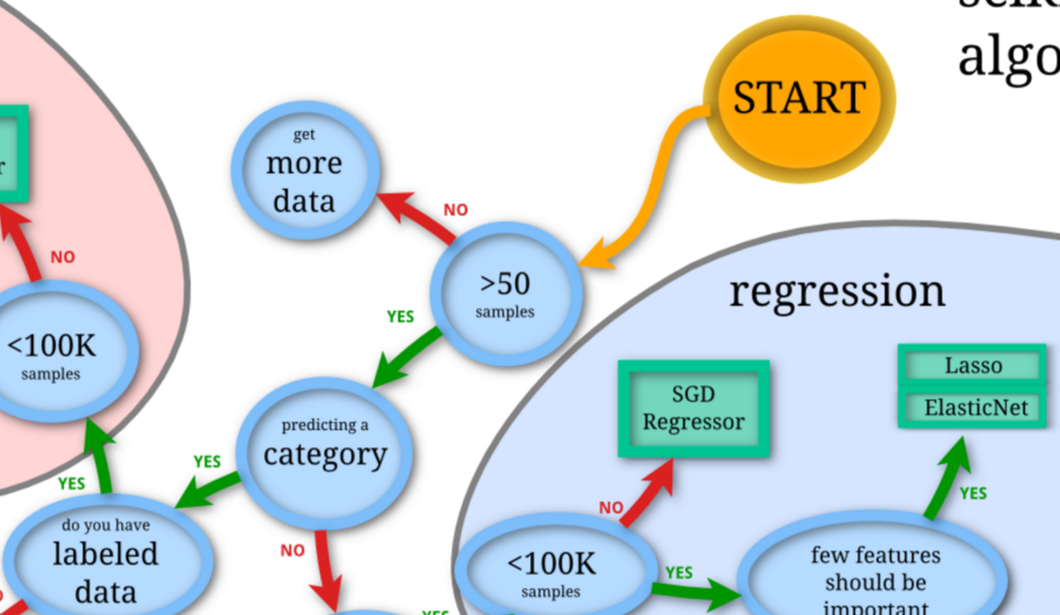
\includegraphics[width=6.5cm]{../pic/scikit_desicion_tree.png}\centering
  \end{center}
  На каждом шаге мы отвечаем на вопрос и "идем по дереву дальше".
  \end{frame}

  \begin{frame}{Пример дерева решений: <<Ирисы Фишера>>}
  \begin{center}
  	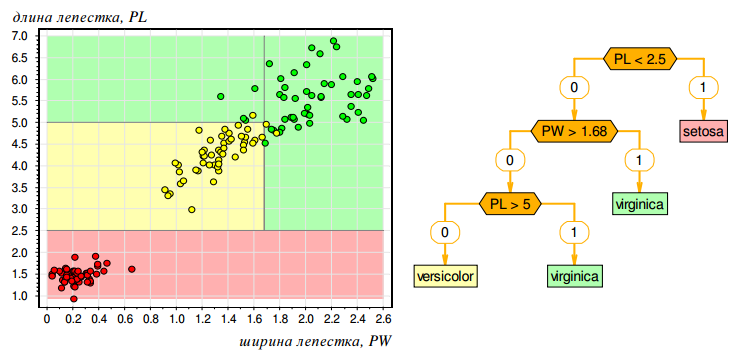
\includegraphics[width=11cm]{../pic/fisher_iris_tree.png}
  \end{center}
  Пример \term{экспертной системы}, являющийся решающим деревом.
  \end{frame}

  \begin{frame}{Пример дерева решений: <<Ирисы Фишера>>}
  
   \begin{center}
  	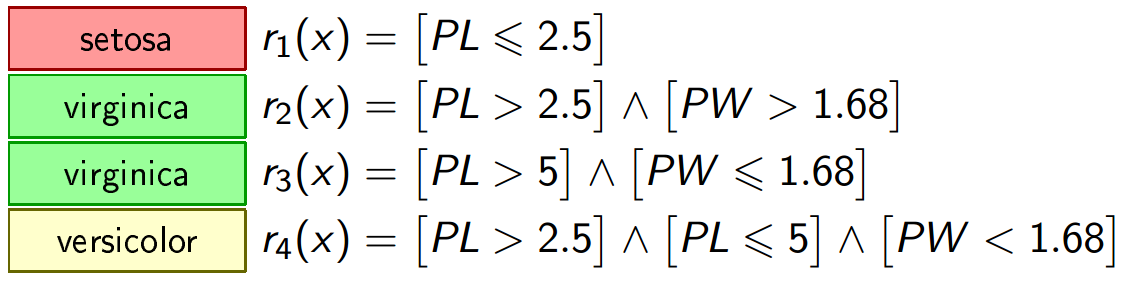
\includegraphics[width=11cm]{../pic/fisher_iris_boolean.png}
  \end{center}
  
  Любое \term{дерево решений} можно представить в виде совокупности
  булевых выражений.
  \end{frame}

  \begin{frame}{Формальное определение}
  
  \termdef{Дерево} -- это \fbox{связанный} \fbox{ациклический} \fbox{граф}.
  
  \termdef{Дерево решений} -- это \fbox{дерево}, в терминальных вершинах которых 
  определён \term{отклик}, в остальных \fbox{листьях} -- функции\footnote{
  	на практике -- \term{булевые} функции, но в общем определении -- не обязательно.}
  каждый выход из которых определяет метку какого-либо выходящего \fbox{ребра}.
  \end{frame}

  \begin{frame}{Лес решений.}
  \termdef{Лес решений} -- это \term{ансамбль}, каждый классификатор которого 
  является \term{деревом решений}.
  
  Обычно лес решений -- это среднее арифметическое всех его деревьев. 
  
  Например решаем задачу обнаружения мошенничества. Всего обучено 500 деревьев решений.
  На какой-либо транзакции 423 дерева определили что эта транзакция мошенническая,
  42 -- легитимная, остальные 35 деревьев -- отказ от классификации.
  
  \auditorium{Каков отклик данного леса?}
  \end{frame}

    \begin{frame}{Лес решений.}
  \termdef{Лес решений} -- это \term{ансамбль}, каждый классификатор которого 
  является \term{деревом решений}.
  
  Обычно лес решений -- это среднее арифметическое всех его деревьев. 
  
  Например решаем задачу обнаружения мошенничества. Всего обучено 500 деревьев решений.
  На какой-либо транзакции 423 дерева определили что эта транзакция мошенническая,
  42 -- легитимная, остальные 35 деревьев -- отказ от классификации.
  
  Тогда лес вернёт решение, что с вероятностью $p=\frac{423}{423+42} = 0,9097$ 
  данная операция является мошеннической.
  \end{frame}

  \section{Построение случайного дерева решений.}\label{section:random_tree_building}

  \begin{frame}
  
  \begin{block}
  	Существует большое количество оптимизаций и улучшений. 
  	Данное описание построения показывает СУТЬ работы. 
  	Желающие понять тему до конца могут ознакомится с академическими работами 
  	по построению современных Random Forest систем.
  \end{block}
  \end{frame}

  \begin{frame}{Постановка задачи}
  Рассмотрим случай, в котором \term{вектор признаков} 
  состоит всего из двух величин: $(x_1, x_2)$.
  
  Таким образом \term{обучающая выборка} $U_{fit}$ имеет вид:
  \begin{equation}
  U_{fit} = \left\{ y \mapsto (x_1, x_2 )\right\}
  \end{equation}
  
  Тогда требуется определить 
  \term{функцию высшего порядка}
  $fit$, которая принимает на
  вход $U_{fit}$ а на выходе возвращает функцию $score$:
  \begin{equation}
  score := fit(U_{fit}) 
  \end{equation}
  
  \fbox{Функция $score$ -- это \term{дерево решений}.}
  
  На выходе $score$ возвращает $\hat{y} \in \{0, 1\}$:
  \begin{equation}
  \hat {y} := score(x_1, x_2)
  \end{equation}
  \end{frame}

  \begin{frame}{Визуализация данных}
  Для удобства обозначим $y=1$ (мошенничество) красным треугольником, 
  $y=0$ (легитимная операция) -- синим кругом.
  
  Так как у нас вектор признаков состоит из двух признаков, то можно визуализировать это на плоскости.
  
  % TODO 
  См. это: http://www.texample.net/tikz/examples/intersecting-lines/
  
  
  \end{frame}
  
  \section{Список материалов}
  
  \begin{frame}{Случайные леса}
  Сергей Павлович Чистяков \textbf{<<Случайные леса: обзор>>}\footnote{\tiny
\url{http://resources.krc.karelia.ru/transactions/doc/trudy2013/trudy_2013_1_117-136.pdf}
}

	\textbf{sklearn}:
	\begin{itemize}
		\item sklearn.ensemble.RandomForestClassifier\footnote{
			\tiny \url{https://scikit-learn.org/stable/modules/generated/sklearn.ensemble.RandomForestClassifier.html}
		}
		\item sklearn.ensemble.RandomForestRegressor\footnote{
			\tiny
			\url{https://scikit-learn.org/stable/modules/generated/sklearn.ensemble.RandomForestRegressor.html}
		}
	    \item sklearn.ensemble.IsolationForest\footnote{
	       \tiny
	       \url{https://scikit-learn.org/stable/modules/generated/sklearn.ensemble.IsolationForest.html}
    	}
	\end{itemize}
  \end{frame}
  
  \section{Вопросы к лекции}
  
  \begin{frame}
  В банковской системе <<ВашБанк Онлайн>> введена система фрод-мониторинга. 
  Она представляет собой лес решений из 700 деревьев решений. Функция принятия решений -- среднее арифметическое. На определённой транзакции 573 деревьев определило транзакцию как мошенническую, 57 как легитимную, остальные -- отказ от классификации.
  \begin{enumerate}
     \item каков отклик системы ФМ?
     \item каков отклик системы ФМ, если отказ от классификации считать легитимными операциями?
     \item каков отклик системы ФМ, если отказ от классификации считать подозрением на мошенничество?
     \item каков отклик системы ФМ, если отказ от классификации считать подозрением на мошенничество, однако вклад брать не как 1, а как 0.7 ?
  \end{enumerate}
  
  \end{frame}
  
  

\end{document}